\documentclass[a4paper,12pt]{article}
\usepackage[a4paper, hmargin={1.5cm,1.5cm}, vmargin={2cm,2cm}]{geometry}
\usepackage{amsmath}
\usepackage{amsthm}
\usepackage{amsfonts}
\usepackage{color}
\usepackage[final]{graphicx}
\usepackage{subcaption}
\usepackage{wrapfig}
\newtheorem{prob}{Problem}[]
\newtheorem{prop}{Proposition}
\usepackage{amssymb}
\usepackage{enumitem}
\usepackage{listings}

\newcommand{\R}{\mathbb{R}}
\newcommand{\C}{\mathbb{C}}
\newcommand{\N}{\mathbb{N}}

\DeclareMathOperator*{\capmod}{\cap}

% Title Page
\title{Basics of Applied Analysis A Report}
\author{Alifian Mahardhika Maulana}


\begin{document}
\maketitle
\begin{prob}
	Discuss the stability of the difference schemes for the transport equation
	\begin{equation}\label{eq:1}
	u_x + bu_x = 0
	\end{equation}
	using von Neumann stability analysis:
	\begin{enumerate}
		\item "naive" explicit scheme
		\begin{equation}\label{eq:2}
		\frac{v_k^{n+1}-v_k^n}{\tau} + b \frac{v_{k+1}^{n}-v_{k-1}^n}{2h} = 0
		\end{equation}
		
		\item implicit scheme
		\begin{equation}\label{eq:3}
		\frac{v_k^{n+1}-v_k^n}{\tau} + b \frac{v_{k+1}^{n+1}-v_{k-1}^{n+1}}{2h} = 0
		\end{equation}
		
		\item Discuss the dissipation and dispersion properties of the implicit scheme in (b). Is it a satisfactory scheme for \eqref{eq:1}
	\end{enumerate}
\end{prob}
\textbf{Answer:}
\begin{enumerate}
	\item von Neumann stability analysis for "naive" explicit scheme:\\
	we rewrite \eqref{eq:2} become,
	\begin{equation}\label{eq:4}
	v_k^{n+1} = v_k^n - \frac{R}{2}(v_{k+1}^n - v_{k-1}^n), \quad R:=\frac{b\tau}{h}
	\end{equation}
	then substitute $v_{k+q} = e^{iq\xi}\hat{v}^n$ to \eqref{eq:4}, we get
	\begin{equation}\label{eq:5}
	\hat{v}^{n+1} = \hat{v}^n \left( 1- \frac{R}{2} (e^{i\xi}-e^{-i\xi}) \right)
	\end{equation}
	then we define, $g(\xi) = \left( 1- \frac{R}{2} (e^{i\xi}-e^{-i\xi}) \right) = 1-iR \sin (\xi)$, taking norm of $g(\xi)$ we get
	\begin{equation}\label{eq:6}
	|g(\xi)| = |1-iR\sin (\xi)| = \sqrt{1+R^2\sin^2(\xi)}, \quad \xi = (-\pi,\pi)
	\end{equation}
	by \eqref{eq:6} we get $|g(\xi)| > 1$, according to von Neumann stability, the explicit scheme \eqref{eq:2} is unstable.
	
	\item von Neumann stability analysis for implicit scheme:\\
	we rewrite \eqref{eq:3} become,
	\begin{equation}\label{eq:7}
	\frac{R}{2} \left(v_{k+1}^{n+1} - v_{k-1}^{n+1}\right) + v_k^{n+1} = v_k^n, \quad R:=\frac{b\tau}{h}
	\end{equation}
	then substitute $v_{k+q} = e^{iq\xi}\hat{v}^n$ to \eqref{eq:7}, we get
	\begin{equation}\label{eq:8}
	\begin{aligned}
	\left(1+\frac{R}{2} \left(e^{i\xi}-e^{-i\xi}\right) \right) \hat{v}^{n+1} &= \hat{v}^{n}\\
	\hat{v}^{n+1} &= \frac{1}{\left(1+\frac{R}{2} \left(e^{i\xi}-e^{-i\xi}\right) \right)} \hat{v}^{n}
	\end{aligned}
	\end{equation}
	then we define, $g(\xi) = \frac{1}{\left(1+\frac{R}{2} \left(e^{i\xi}-e^{-i\xi}\right) \right)} = \frac{1}{\left(1+iR\sin(\xi) \right)}$, taking norm of $g(\xi)$ we get
	\begin{equation}\label{eq:9}
	|g(\xi)| = \Bigr|\frac{1}{\left(1+iR\sin(\xi) \right)}\Bigr| = \frac{1}{\sqrt{1+R^2 \sin^2 (\xi)}}, \quad \xi = (-\pi,\pi)
	\end{equation}
	by \eqref{eq:9} we get $|g(\xi)| < 1$, according to von Neumann stability, the implicit scheme \eqref{eq:3} is stable.
	
	\item To analyze the dissipation and dispersion of \eqref{eq:3}, we substitute $v_{k+p}^{n+q} = e^{i(q\omega\tau + p\beta h)}$ to \eqref{eq:7} we get,
	\begin{equation}\label{eq:10}
	\begin{aligned}
	\frac{R}{2} \left(e^{i(\omega\tau + \beta h)} - e^{i(\omega\tau - \beta h)}\right) + e^{i\omega\tau} &= 1, \quad R:=\frac{b\tau}{h}\\
	\left(\frac{R}{2} \left(e^{i\beta h} - e^{-i\beta h}\right) + 1 \right) e^{i\omega \tau} &= 1\\
	\left(iR\sin(\beta h) + 1\right) e^{i\omega \tau} &= 1\\
	e^{i\omega \tau} &= \frac{1}{\left(iR\sin(\beta h) + 1\right)}
	\end{aligned}
	\end{equation}
	taking norm of $e^{i\omega \tau}$, we get
		\begin{equation}\label{eq:11}
		|e^{i\omega \tau}| = e^{-\omega_2\tau} = \frac{1}{R^2\sin^2(\beta h) + 1}
		\end{equation}
	by \eqref{eq:11}, $e^{-\omega_2\tau} < 1$, therefore according to von Neumann stability analysis, the implicit scheme on \eqref{eq:3} is \textbf{dissipative}.\\
	Then, to analyze the dispersion, we take $\arg(e^{i\omega\tau})$,
	\begin{equation}\label{eq:12}
	\begin{aligned}
	\arg(e^{i\omega\tau}) &= \arg(e^{i\omega_1\tau}) + \arg(e^{-\omega_2\tau})\\
	&= \omega_1\tau + 0
	\end{aligned}
	\end{equation}
	which, $\omega_1\tau = \arctan\left(\frac{Im(e^{i\omega \tau})}{Re(e^{i\omega \tau})}\right)$, we can get the real and imajiner part of $e^{i\omega \tau}$ by first multiplying it with it's rational factor,
	\begin{equation}\label{eq:13}
	e^{i\omega \tau} = \frac{1}{\left(iR\sin(\beta h) + 1\right)} \frac{\left(iR\sin(\beta h) - 1\right)}{\left(iR\sin(\beta h) - 1\right)} = -\frac{iR\sin(\beta h)+1}{R^2\sin^2+1}
	\end{equation}
	then, $\omega_1\tau = \arctan\left(\frac{Im(e^{i\omega \tau})}{Re(e^{i\omega \tau})}\right) = \frac{R\sin(\beta h)}{1}=R\sin(\beta h)$. Since $\omega_1\tau$ is not a constant, therefore, according to von Neumann stability analysis, the implicit scheme on \eqref{eq:3} is \textbf{dispersive}.
\end{enumerate}
\newpage
\begin{prob}
	Show that the following implicit difference schemes for approximating the solution to
	\begin{equation}
	u_t + bu_x = au_{xx}
	\end{equation}
	are unconditionally stable using the von Neumann stability analysis. Here $R = b\frac{\tau}{h},r=a\frac{\tau}{h^2}$.
	\begin{enumerate}
		\item \begin{equation}\label{eq:15}
		v_{k}^{n+1} + \frac{R}{2}(v_{k+1}^{n+1}-v_{k-1}^{n+1}) - r(v_{k+1}^{n+1}-2v_{k}^{n+1} + v_{k-1}^{n+1}) = v_{k}^{n}
		\end{equation}
		\item \begin{equation}\label{eq:16}
		v_{k}^{n+1} + \frac{R}{4}(v_{k+1}^{n+1}-v_{k-1}^{n+1}) - \frac{r}{2}(v_{k+1}^{n+1}-2v_{k}^{n+1} + v_{k-1}^{n+1}) = v_{k}^{n} - \frac{R}{4}(v_{k+1}^{n}-v_{k-1}^{n}) + \frac{r}{2}(v_{k+1}^{n}-2v_{k}^{n} + v_{k-1}^{n})
		\end{equation}
	\end{enumerate}
\end{prob}
\textbf{Answer:}
\begin{enumerate}
	\item Substitute $v_{k+q}=e^{iq\xi}\hat{v}^n$ to \eqref{eq:15} we get,
	\begin{equation}\label{eq:17}
	\begin{aligned}
	\hat{v}^{n+1} + \frac{R}{2}(e^{i\xi} - e^{-i\xi}) \hat{v}^{n+1} - r(e^{i\xi}-2+e^{-i\xi})\hat{v}^{n+1} = \hat{v}^n\\
	\hat{v}^{n+1} \bigg( 1 + \frac{R}{2}(e^{i\xi} - e^{-i\xi}) - r(e^{i\xi}-2+e^{-i\xi}) \bigg) = \hat{v}^n\\
	\hat{v}^{n+1} = \frac{1}{\bigg( 1 + \frac{R}{2}(e^{i\xi} - e^{-i\xi}) - r(e^{i\xi}-2+e^{-i\xi}) \bigg)} \hat{v}^n
	\end{aligned}
	\end{equation}
	then, we define:
	\begin{equation}\label{eq:18}
	\begin{aligned}
	g(\xi) &= \frac{1}{\bigg( 1 + \frac{R}{2}(e^{i\xi} - e^{-i\xi}) - r(e^{i\xi}-2+e^{-i\xi}) \bigg)} = \frac{1}{\bigg(1+iR\sin(\xi) +r(2\cos(\xi)-2)\bigg)}\\ 
	&=\frac{1}{\bigg(1+iR\sin(\xi) +r(-4\sin^2(\frac{\xi}{2}))\bigg)}
	\end{aligned}
	\end{equation}
	by \eqref{eq:18}, $g(\xi)<1$, according to von Neumann stability analysis, if $g(\xi)<1$ the scheme will be unconditionally stable.
	
	\item Substitute $v_{k+q}=e^{iq\xi}\hat{v}^n$ to \eqref{eq:16} we get,
	\begin{equation}\label{eq:19}
	\begin{aligned}
	\hat{v}^{n+1} + \frac{R}{4}(e^{i\xi} - e^{-i\xi}) \hat{v}^{n+1} - \frac{r}{2}(e^{i\xi}-2+e^{-i\xi})\hat{v}^{n+1} &= \hat{v}^n -\frac{R}{4}(e^{i\xi} - e^{-i\xi}) \hat{v}^{n} +\frac{r}{2}(e^{i\xi}-2+e^{-i\xi})\hat{v}^{n}\\
	\hat{v}^{n+1} \bigg( 1 + \frac{R}{4}(e^{i\xi} - e^{-i\xi})- \frac{r}{2}(e^{i\xi}-2+e^{-i\xi}) \bigg) &= \hat{v}^n
	\bigg( 1 -\frac{R}{4}(e^{i\xi} - e^{-i\xi}) +\frac{r}{2}(e^{i\xi}-2+e^{-i\xi}) \bigg)\\
	\hat{v}^{n+1} &= \frac{\bigg( 1 -\frac{R}{4}(e^{i\xi} - e^{-i\xi}) +\frac{r}{2}(e^{i\xi}-2+e^{-i\xi}) \bigg)}{\bigg( 1 + \frac{R}{4}(e^{i\xi} - e^{-i\xi})- \frac{r}{2}(e^{i\xi}-2+e^{-i\xi}) \bigg)}\hat{v}^n
	\end{aligned}
	\end{equation}
	then, we define:
	\begin{equation}\label{eq:20}
	\begin{aligned}
	g(\xi) &= \frac{\bigg( 1 -\frac{R}{4}(e^{i\xi} - e^{-i\xi}) +\frac{r}{2}(e^{i\xi}-2+e^{-i\xi}) \bigg)}{\bigg( 1 + \frac{R}{4}(e^{i\xi} - e^{-i\xi})- \frac{r}{2}(e^{i\xi}-2+e^{-i\xi}) \bigg)} = \frac{\bigg( 1 -\frac{R}{4}(2i\sin(\xi)) +\frac{r}{2}(2\cos(\xi)-2) \bigg)}{\bigg( 1 + \frac{R}{4}(2i\sin(\xi))- \frac{r}{2}(2\cos(\xi)-2) \bigg)}\\ 
	&=\frac{\bigg( 1 -\frac{R}{4}(2i\sin(\xi)) +\frac{r}{2}(-4\sin^2(\frac{\xi}{2})) \bigg)}{\bigg( 1 + \frac{R}{4}(2i\sin(\xi))- \frac{r}{2}(-4\sin^2(\frac{\xi}{2})) \bigg)}
	\end{aligned}
	\end{equation}
	by \eqref{eq:20}, $g(\xi)<1$, according to von Neumann stability analysis, if $g(\xi)<1$ the scheme will be unconditionally stable.
\end{enumerate}

\begin{prob}
	Discuss the dissipation and dispersion of the following implicit numerical schemes for the wave equation
	\begin{enumerate}
		\item \begin{equation}\label{eq:21}
		\frac{v_k^{n+1} -2v_k^n+v_k^{n-1}}{\tau^2} = \frac{v_{k+1}^{n+1}-2v_k^{n+1}+v_{k-1}^{n+1}}{h^2}
		\end{equation}
		\item \begin{equation}\label{eq:22}
		\frac{v_k^{n+1} -2v_k^n+v_k^{n-1}}{\tau^2} = \frac{v_{k+1}^{n+1}-2v_k^{n+1}+v_{k-1}^{n+1}}{2h^2} + \frac{v_{k+1}^{n-1}-2v_k^{n-1}+v_{k-1}^{n-1}}{2h^2}
		\end{equation}
	\end{enumerate}
\end{prob}
\textbf{Answer:}
\begin{enumerate}
	\item Substitute $v_{k+p}^{n+q} = e^{i(q\omega\tau + p\beta h)}\hat{v}^n$ with $R=\frac{\tau}{h}$ to \eqref{eq:21} we get,
	\begin{equation}\label{eq:23}
	\begin{aligned}
	\frac{(e^{i\omega\tau} -2 + e^{-i\omega\tau})}{\tau^2}\hat{v}^n &= \frac{(e^{i(\omega\tau+\beta h)}-2e^{i\omega\tau}+e^{i(\omega\tau-\beta h)})}{h^2}\hat{v}^n\\
	e^{i\omega\tau} -2 + e^{-i\omega\tau} &= R^2(2\cos(\beta h)-2)e^{i\omega\tau}\\
	\end{aligned}
	\end{equation}
	take $g=e^{i\omega\tau}$, \eqref{eq:23} become
	\begin{equation}
	\begin{aligned}
	-2 + g^{-1} + g\left(1 - R^2(2\cos(\beta h)-2)\right) &= 0\\
	-2 + g^{-1} + g\left(1 - R^2(-4\sin^2(\frac{\beta h}{2}))\right) &= 0\\
	\end{aligned}
	\end{equation}
	multiple by $g$ we get
	\begin{equation}\label{eq:25}
	\begin{aligned}
	g^2(1-R^2(-4\sin^2(\frac{\beta h}{2}))) -2g + 1 = 0
	\end{aligned}
	\end{equation}
	solving \eqref{eq:25} we get,
	\begin{equation}\label{eq:26}
	g = e^{i\omega\tau} = \frac{1\pm i2R\sin(\frac{\beta h}{2})}{(1-R^2(-4\sin^2(\frac{\beta h}{2})))}
	\end{equation}
	taking norm of \eqref{eq:26}, we get
	\begin{equation}\label{eq:27}
	|e^{i\omega\tau}| = e^{i\omega_2\tau} = \max_{-\pi \leq \frac{\beta h}{2} \leq \pi} \left| \frac{1\pm i2R\sin(\frac{\beta h}{2})}{(1-R^2(-4\sin^2(\frac{\beta h}{2})))} \right| = \frac{1\pm 2R}{1+4R^2}
	\end{equation}
	from \eqref{eq:27}, $e^{i\omega_2\tau} < 1$, therefore according to von Neumann stability analysis, the implicit numerical scheme on \eqref{eq:21} is \textbf{dissipative}.
	
	Then, to analyze the dispersion, we take $\arg(e^{i\omega\tau})$,
	\begin{equation}\label{eq:28}
	\begin{aligned}
	\arg(e^{i\omega\tau}) &= \arg(e^{i\omega_1\tau}) + \arg(e^{-\omega_2\tau})\\
	&= \omega_1\tau + 0
	\end{aligned}
	\end{equation}
	which, $\omega_1\tau = \arctan\left(\frac{Im(e^{i\omega \tau})}{Re(e^{i\omega \tau})}\right)$,
	then, $\omega_1\tau = \arctan\left(\frac{Im(e^{i\omega \tau})}{Re(e^{i\omega \tau})}\right) = \frac{2R\sin(\beta h)}{1}=2R\sin(\beta h)$. Since $\omega_1\tau$ is not a constant, therefore, according to von Neumann stability analysis, the implicit scheme on \eqref{eq:21} is \textbf{dispersive}.
	
	\item Substitute $v_{k+p}^{n+q} = e^{i(q\omega\tau + p\beta h)}\hat{v}^n$ with $R=\frac{\tau^2}{2h^2}$ to \eqref{eq:22} we get,
	\begin{equation}\label{eq:29}
	\begin{aligned}
	&\frac{(e^{i\omega\tau} -2 + e^{-i\omega\tau})}{\tau^2}\hat{v}^n = \frac{(e^{i(\omega\tau+\beta h)}-2e^{i\omega\tau}+e^{i(\omega\tau-\beta h)})}{2h^2}\hat{v}^n + \frac{(e^{i(-\omega\tau+\beta h)}-2e^{-i\omega\tau}+e^{-i(\omega\tau+\beta h)})}{2h^2}\hat{v}^n\\
	&(e^{i\omega\tau}-2+e^{-i\omega\tau}) = R \left( (2\cos(\beta h)-2)e^{i\omega\tau} + (2\cos(\beta h)-2)e^{-i\omega\tau} \right)\\
	&(e^{i\omega\tau}-2+e^{-i\omega\tau}) - R \left( (2\cos(\beta h)-2)e^{i\omega\tau} + (2\cos(\beta h)-2)e^{-i\omega\tau} \right) = 0\\
	&e^{i\omega\tau} \left( 1- R (2\cos(\beta h)-2)\right) + e^{-i\omega\tau} \left( 1- R (2\cos(\beta h)-2)\right) -2 = 0
	\end{aligned}
	\end{equation}
	take $g=e^{i\omega\tau}$, \eqref{eq:29} become
	\begin{equation}
	\begin{aligned}
	g \left( 1- R (2\cos(\beta h)-2)\right) + g^{-1} \left( 1- R (2\cos(\beta h)-2)\right) -2 = 0\\
	g \left( 1- R (-4\sin^2(\frac{\beta h}{2})\right) + g^{-1} \left( 1- R (-4\sin^2(\frac{\beta h}{2})\right) -2 = 0\\
	\end{aligned}
	\end{equation}
	multiple by $g$, we get
	\begin{equation}\label{eq:31}
	g^2 \left( 1- R (-4\sin^2(\frac{\beta h}{2})\right) + \left( 1- R (-4\sin^2(\frac{\beta h}{2})\right) -2g = 0
	\end{equation}
	solving \eqref{eq:31} we get,
	\begin{equation}\label{eq:32}
	g = e^{i\omega\tau} = \frac{2\pm \sqrt{4-4(1+4R\sin^2(\frac{\beta h}{2}))^2}}{2(1+4R\sin^2(\frac{\beta h}{2}))}
	\end{equation}
	taking norm of \eqref{eq:32}, we get
	\begin{equation}\label{eq:33}
	|e^{i\omega\tau}| = e^{i\omega_2\tau} = \max_{-\pi \leq \frac{\beta h}{2} \leq \pi} \left| \frac{2\pm \sqrt{4-4(1+4R\sin^2(\frac{\beta h}{2}))^2}}{2(1+4R\sin^2(\frac{\beta h}{2}))} \right| = \frac{2\pm (1+4R)}{2(1+4R)}
	\end{equation}
	from \eqref{eq:33}, $e^{i\omega_2\tau} = 1$, therefore according to von Neumann stability analysis, the implicit numerical scheme on \eqref{eq:22} is \textbf{non-dissipative}.
	
	Then, to analyze the dispersion, we take $\arg(e^{i\omega\tau})$,
	\begin{equation}\label{eq:28}
	\begin{aligned}
	\arg(e^{i\omega\tau}) &= \arg(e^{i\omega_1\tau}) + \arg(e^{-\omega_2\tau})\\
	&= \omega_1\tau + 0
	\end{aligned}
	\end{equation}
	which, $\omega_1\tau = \arctan\left(\frac{Im(e^{i\omega \tau})}{Re(e^{i\omega \tau})}\right)$,
	then, $\omega_1\tau = \arctan\left(\frac{Im(e^{i\omega \tau})}{Re(e^{i\omega \tau})}\right) = 0$. Since $\omega_1\tau$ is 0 because there is no imaginer part, therefore, according to von Neumann stability analysis, the implicit scheme on \eqref{eq:22} is \textbf{non-dispersive}.
\end{enumerate}
\newpage
\begin{prob}
	Implement the "naive" finite difference scheme and the implicit scheme to solve
	\begin{equation}\label{eq:35}
	\begin{cases}
	u_t + u_x = 0 \quad \text{in}\ (0,1) x (0,\infty)\\
	u(x,0) = f(x) \quad \text{for}\ x\in (0,1)\\
	u(0,t) = 0 \quad \text{for}\ t\geq 0
	\end{cases}
	\end{equation}
\end{prob}
\textbf{Answer:}
\begin{enumerate}
	\item Exact Solution: We want to find the exact solution of \eqref{eq:35} using general solution $$u(x,t) = f(x)(x-t)$$
	\begin{enumerate}
		\item For \begin{equation*}
		f(x) = \begin{cases}
		0.25 - |x - 0.25|, \quad x<0.5\\
		0, \quad x\geq0.5
		\end{cases}
		\end{equation*} we have the exact solution as follow:
		\begin{equation}
		u(x,t) = (0.25-|x-0.25|)(x-t)
		\end{equation}
		
		\item For $$f(x)=xe^{-100(x-0.25)^2}$$ the exact solution is:
		\begin{equation}
		u(x,t) = (x^2-xt)e^{-100(x-0.25)^2}
		\end{equation}
	\end{enumerate}
\item Error plot for naive scheme with error defined by:
\begin{equation*}
\max_{0<k<M} |v_k^n-u(kh,n\tau)|
\end{equation*}
\begin{figure}[h!]
	\begin{subfigure}{0.49\linewidth}
		\centering
		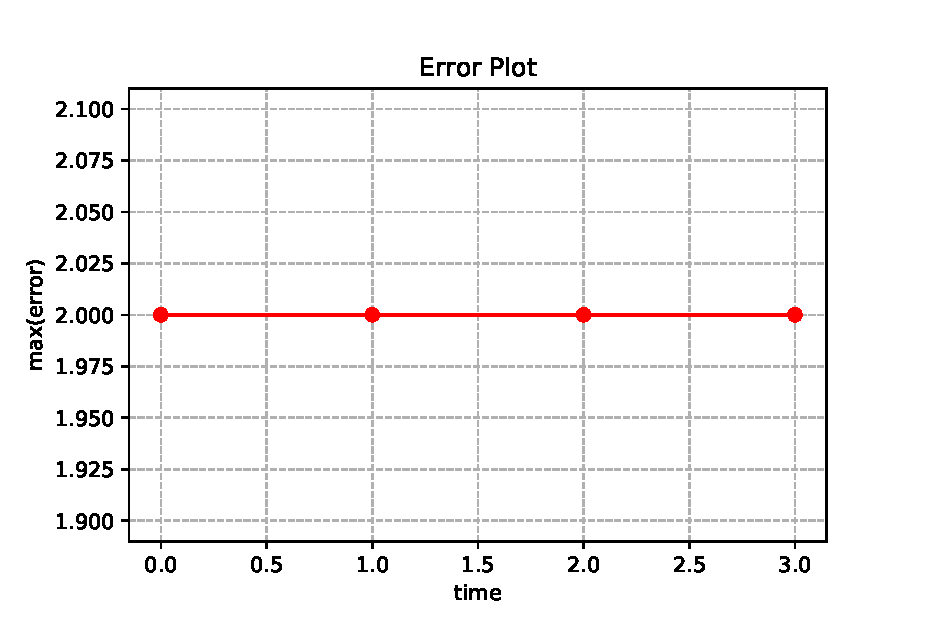
\includegraphics[width=\linewidth]{baapict/errori}
		\caption{Error Plot using (i) initial data}
	\end{subfigure}
\begin{subfigure}{0.49\linewidth}
	\centering
	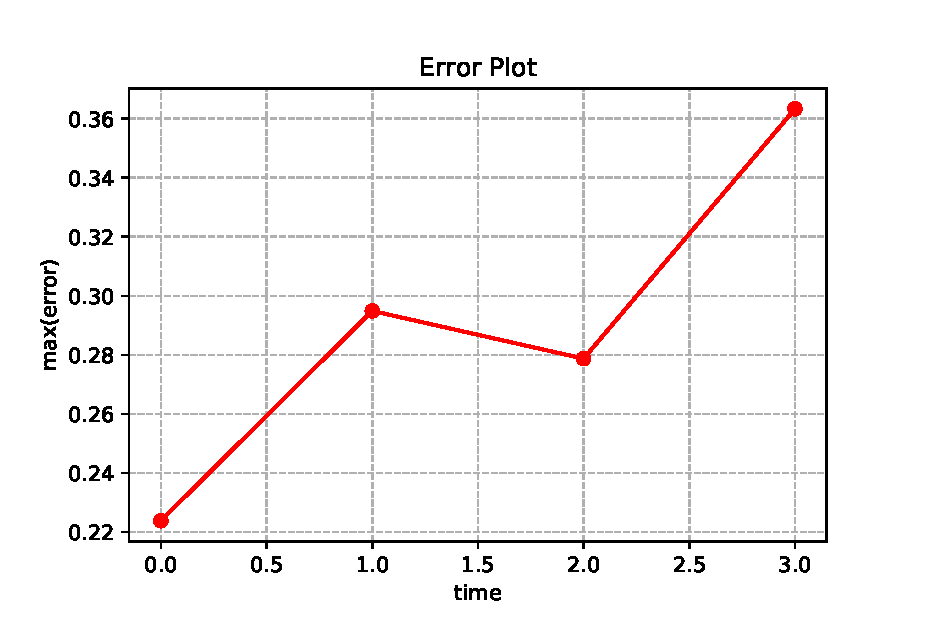
\includegraphics[width=\linewidth]{baapict/errorii}
	\caption{Error Plot using (ii) initial data}
\end{subfigure}
\end{figure}\\
\newline
Error Plot for Implicit Scheme:
\begin{figure}[h!]
	\begin{subfigure}{0.49\linewidth}
		\centering
		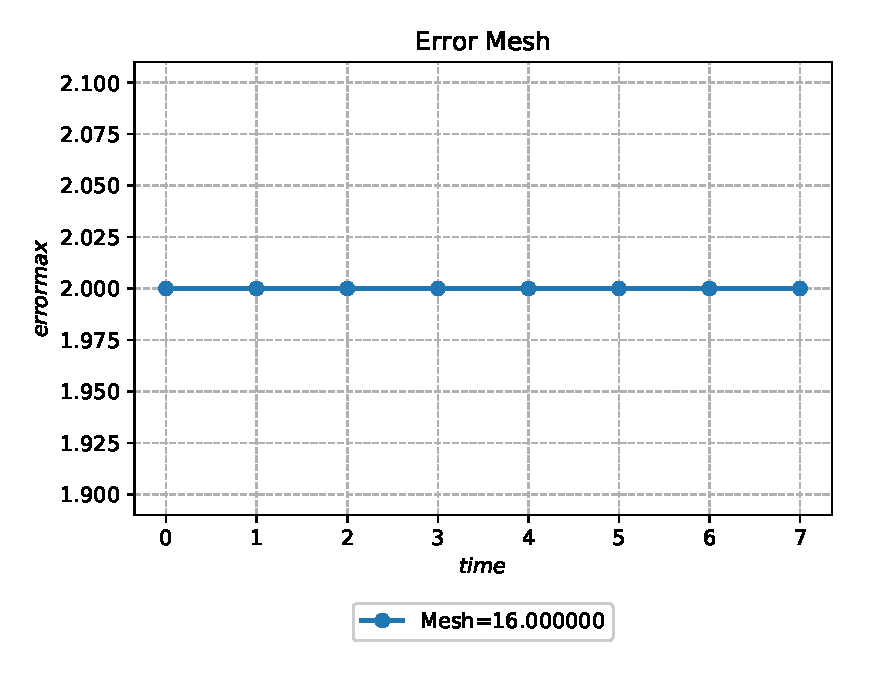
\includegraphics[width=\linewidth]{baapict/errmeshimpi}
		\caption{Error Plot using (i) initial data for implicit scheme}
	\end{subfigure}
	\begin{subfigure}{0.49\linewidth}
		\centering
		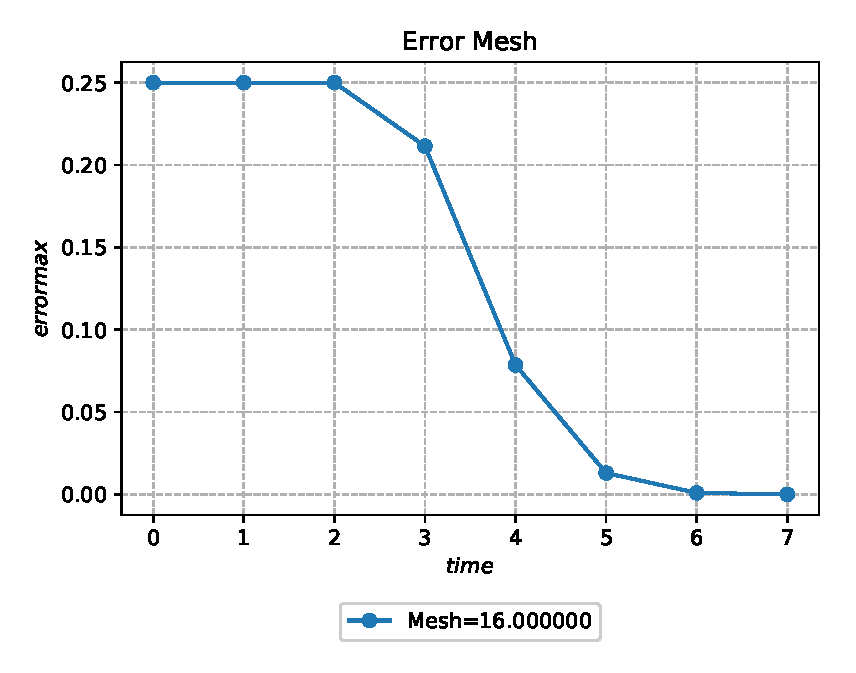
\includegraphics[width=\linewidth]{baapict/errmeshimpii}
		\caption{Error Plot using (ii) initial data for implicit scheme}
	\end{subfigure}
\end{figure}
\newpage
\item Check the maximum error in the naive scheme
\item Is the error increasing with the same rate if use the initial condition (ii) above?
\textbf{Answer:} The error is not increasing if using the initial condition (ii), vice versa, the solution is better if using initial condition (ii)

\item How does the maximum of the error behave if the mesh size $M=128,256,512$?
As shown in the figure below, using "naive" scheme, the solution always blowup, at the other han, using implicit scheme, resulting in stable and convergent result.
\begin{figure}[h!]
	\begin{subfigure}{0.49\linewidth}
		\centering
		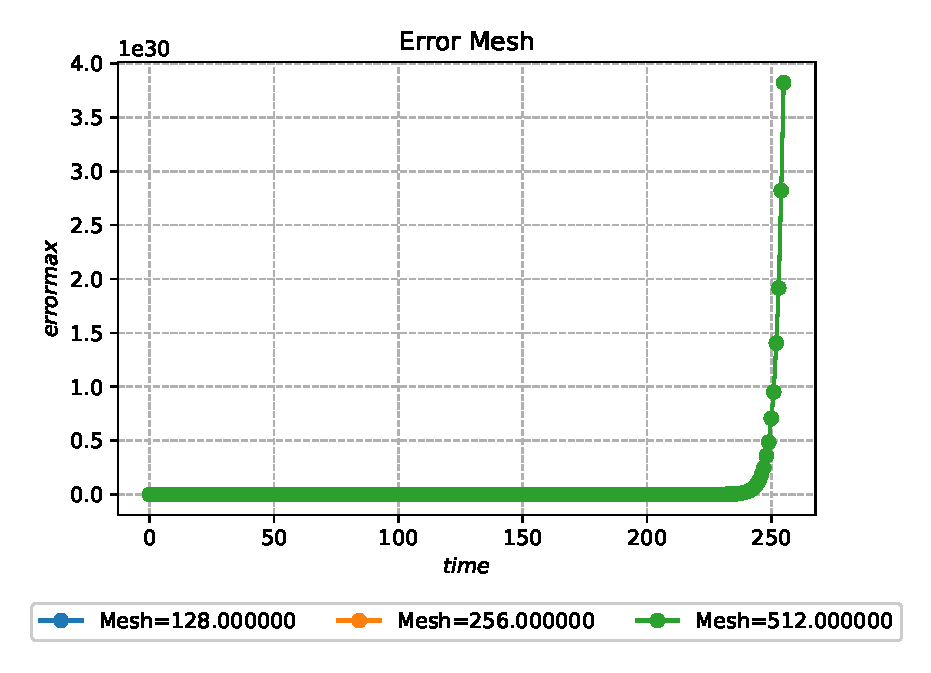
\includegraphics[width=\linewidth]{baapict/errmesh}
		\caption{Error plot overtime in Naive Scheme}
	\end{subfigure}
	\begin{subfigure}{0.49\linewidth}
		\centering
		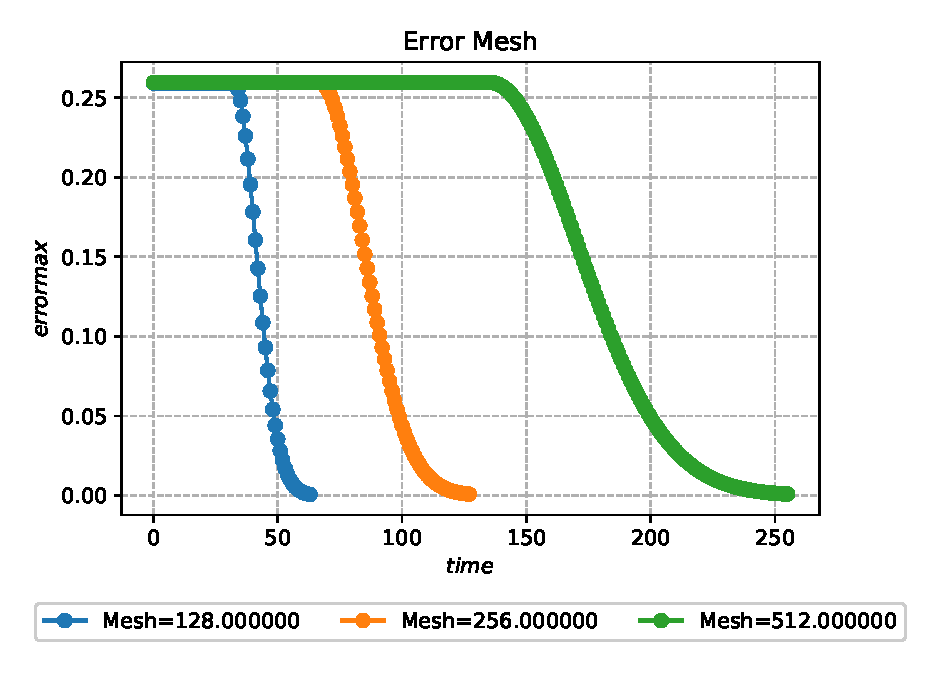
\includegraphics[width=\linewidth]{baapict/errmeshimplicit}
		\caption{Error plot overtime in Implicit Scheme}
	\end{subfigure}
\end{figure}
\end{enumerate}
\end{document}